
\chapter{Introduction}
\label{ch1}

 %%%%%%%%%%%%%%%%%%%%%% POWER BI %%%%%%%%%%%%%%%%%%%%%ù
\section{Power BI}

\begin{figure}[h]
    \centering
    
\includegraphics[width=2.0in, height=2.0in]{Figure/power bi.jpg}
    \caption{Power BI }
    \label{fig:enter-label}
\end{figure}

Power BI is a business analytics service provided by Microsoft. It aims to provide interactive visualizations and business intelligence capabilities to create their own reports and
dashboards for the end users. Our data may be in an Excel spreadsheet, or a collection of a cloud based .Pbix file which is designed for to use with Power BI desktop.
\\ 
Power BI was initially released in 2014, operating system: Microsoft windows. It provides cloud- based services, along with desktop interface, called Power BI Desktop. The key components of the Power BI are (The first one was used in this project): 
\begin{itemize}
    \item Power BI desktop: designing and publishing reports and dashboards to the service.
    \item Power BI service: software as a service.
    \item Power BI mobile apps: iOS, android, and windows phones.
\end{itemize}
Power BI is used for data visualization, analysis, and reporting. It enables users to transform raw data into interactive and visually appealing dashboards and reports, allowing organizations to gain insights and make data-driven decisions.

%%%%%%%%%%%%%%%%%%%%%%% USE CASES %%%%%%%%%%%%%%%%%%%%%%%%
\subsection{Power BI use cases}
The platform's ability to synthesize data from various sources makes it useful for analyzing and reporting data that's culled using an array of tools and methods. Some of the ways different industry sectors use Power BI to their advantage include the following:
\begin{enumerate}
    \item \textbf{Retail:} Reports based on customer purchase data give retailers insight into which products to prioritize and stock.
    \item \textbf{Manufacturing and engineering:} Power BI dashboards are used for process monitoring and reporting resource use. For instance, manufacturing data collected with IoT devices can be analyzed using Power BI. \\
    \item \textbf{Education:} Tracking student performance with Power BI reports and dashboards helps school administrators and teachers identify where improvements are needed.
    \item \textbf{Finance and insurance:} Power BI is conducive to analyzing the large-scale data sets the financial sector uses. The insurance industry can use reports and dashboards to get insight into risk assessments.
\end{enumerate}

%%%%%%%%%%%%%%%%%%%%%%% flow process %%%%%%%%%%%%%%%%%%%%%%%
\subsection{Understanding the Process Flow in Power BI}

\begin{figure}[h]
    \centering
    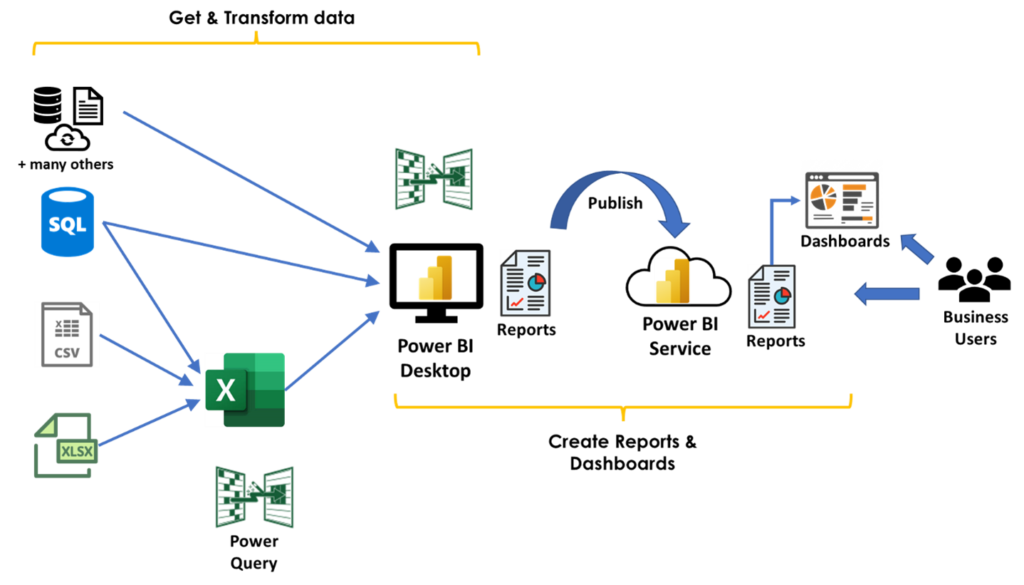
\includegraphics[width=5.0in, height=3.0in]{Figure/Power_BI_Process.png}
    \caption{Process flow in power BI }
    \label{fig:enter-label}
   \textit{Source:} \href{https://sqlspreads.com/blog/power-bi-dashboards-examples-use-cases/}{sqlspreads.com}
\end{figure}

The process flow in Power BI involves several key steps. Initially, data is collected from diverse sources such as databases, spreadsheets, and web services. This data is then transformed, cleaned, and prepared for analysis. Users define relationships between different data tables to create data models that serve as the foundation for analysis. With the data model in place, interactive reports and dashboards are created to visualize the data effectively. Users can then analyze the data to uncover insights, trends, and patterns. These insights can be shared with colleagues and stakeholders for collaborative decision-making. Finally, Power BI solutions are deployed and managed in a production environment to ensure scalability and reliability.

%%%%%%%%%%%%%%%%%%%%%%%% ADV / DIS %%%%%%%%%%%%%%%%%%%%%%%%



%%%%%%%%%%%%%%%%%%%%%%%% Benifits of power bi dash %%%%%%%%%%%%
\section{Benifits of Power BI dashboards}

Power BI Dashboards are an effective way to convey important high-level information about an area of a business or organization.  They are great at quickly answering critical business questions like \textit{“How is our business doing?”}; \textit{“Are we making our target?”}; \textit{“In which area(s) are we doing well/badly?”}.  Dashboards won’t, however,  help you answer the \textit{“whys”} behind those questions – for those, you need to drill through to the underlying reports and analyze those.\\
A good dashboard can therefore provide the following benefits:

\begin{itemize}
    \item Improved real-time visibility into business performance
    \item Quicker response times when problems arise
    \item Greater transparency
    \item Improved communication across the organization
    \item Time-savings
\end{itemize}

%%%%%%%%%%%%%%%%%%%%%%%%%%%%%%%%%%%%%%%%%%%%%%%%%%%%%%%%%%%%%%%%%%%



























































